\documentclass{article}
\usepackage{graphicx} % Required for inserting images

\title{Informe TFG}
\author{Andrés García Treviño}
\date{April 2026}

\usepackage[left=3cm, right=3cm, top=2cm, bottom=2cm]{geometry}
\usepackage{csvsimple}
\usepackage{booktabs}
\usepackage{longtable}
\usepackage{xcolor}
\usepackage{listings}
\usepackage{placeins}
\usepackage{amsmath}

% Define custom colors
\definecolor{codegreen}{rgb}{0,0.6,0}
\definecolor{codegray}{rgb}{0.5,0.5,0.5}
\definecolor{codepurple}{rgb}{0.58,0,0.82}
\definecolor{backcolour}{rgb}{0.95,0.95,0.92}

% Define the Python style
\lstdefinestyle{pythonstyle}{
    backgroundcolor=\color{backcolour},
    commentstyle=\color{codegreen},
    keywordstyle=\color{magenta},
    numberstyle=\tiny\color{codegray},
    stringstyle=\color{codepurple},
    basicstyle=\ttfamily\footnotesize,
    breakatwhitespace=false,
    breaklines=true,
    captionpos=b,
    keepspaces=true,
    numbers=left,
    numbersep=5pt,
    showspaces=false,
    showstringspaces=false,
    showtabs=false,
    tabsize=2,
    language=Python
}
\setlength{\parindent}{0pt}
\setlength{\parskip}{1em}


\begin{document}

\maketitle

\section{Revisión del código original}
\subsection{Capas de la red neuronal}
La red neuronal inicial era una red LSTM de 1 capa de 24 neuronas y una capa final de 3 neuronas completamente conectadas (\texttt{Dense}).

Para permitir la compatibilidad con otras capas de neuronas y otros entornos de ejecución como Google Colab o Kaggle, he añadido una primera capa de entrada (\texttt{Input}) para establecer el tamaño de los \textit{batches} (\texttt{batch\_input\_size}).

\begin{lstlisting}[style=pythonstyle, caption={Capa \texttt{Input} en la red CNN+LSTM}]

    # CNN-LSTM MODEL
    myCNNLSTM = Sequential()
    myCNNLSTM.add(Input(batch_shape=(batch_size, look_back, 7, 7, 1)))
    myCNNLSTM.add(TimeDistributed(Conv2D(filters=current_filters, kernel_size=(3,3), padding='same', activation='relu')))
    myCNNLSTM.add(TimeDistributed(Flatten())) # Flatten to connect CNN to LSTM
    myCNNLSTM.add(LSTM(look_back, stateful=True))
    myCNNLSTM.add(Dense(num_features))
    myCNNLSTM.compile(loss='mean_squared_error', optimizer='adam')
\end{lstlisting}

\subsection{\textit{Data leakage} por normalización}
En el modelo original se utilizan todas las muestras del dataset para generar el objeto \texttt{MinMaxScaler} con el que se realiza la normalización de los datos. Esto constituye en sí mimo \textit{data leakage}.
\begin{lstlisting}[style=pythonstyle, caption={\textit{Data leakage} original}]
# normalize the dataset
scaler = MinMaxScaler(feature_range=(0, 1))
dataset = scaler.fit_transform(dataset)
\end{lstlisting}

El objetivo del paper SKIMA y de el presente TFG es comparar el entrenamiento incremental \textit{online learning} con el entrenamiento estático. Si la red se entrena primeramente pasando 400 veces (\texttt{n\_epochs}) por el subset de entrenamiento (\texttt{train}), el subset de test (\texttt{test}) no puede estar incluido en la generación del obketo sklearn.preprocessing.\texttt{MinMaxScaler} puesto que la red neuronal estaría preparada de antemano para dicho subset de test y daría unos resultados mejores de los reales.

Además, el entrenamiento de la red neuronal está pensado para desplegar dicha red en un entorno real. En dicho escenario, los datos nuevos que tenga que procesar la red neuronal no podrían generar el objeto \texttt{MinMaxScaler}. Si pudieran, aun así habría que reentrenar la red neuronal cada vez que llegara un nuevo dato.

Lo mismo ocurre con el entrenamiento incremental. Está pensado para que, al desplegar la red neuronal en un entorno real, ésta vaya adaptándose a los cambios en los patrones de tráfico, evitando así caer en el \textit{concept drift} y tener que reentrenar la red neuronal. Los nuevos datos que la red tenga que procesar en dicho escenario no van a generar el objeto \texttt{MinMaxScaler}, por lo tanto, los datos de test tampoco.

Así, he cambiado el script de python de esta forma:

\begin{lstlisting}[style=pythonstyle, caption={Escalado del dataset sin data leakage}]
    dataset = dataset_full[0:train_size+test_size]

    scaler = MinMaxScaler(feature_range=(0, 1))
    train = dataset[0:train_size, :]
    test = dataset[train_size : train_size+test_size, :]

    # se escala sin los datos de test. NO DATA LEAKAGE
    train = scaler.fit_transform(train)
    test = scaler.transform(test)
\end{lstlisting}
%%https://scikit-learn.org/stable/common_pitfalls.html

Los resultados sin \textit{data leakage} corrigen las estimaciones optimistas del test estático con \textit{data leakage}. Esto es porque la red tiene información sobre el set de \texttt{test} en su entrenamiento, lo que mejora falsamente la precisión de sus predicciones. Por ello, el RNMSE estático es menor con \textit{data leakage}. Este es el principal argumento para eliminar el \textit{data leakage}.

No ocurre lo mismo para el entrenamiento incremental, que aumenta su precisión sin el \textit{data leakage}. Mi hipótesis es que, como la red deja de tener información previa sobre el conjunto de \texttt{test}, la actualización de los pesos es más precisa. Por ejemplo, si el conjunto de \texttt{train} tiene un máximo de 1 y el de \texttt{test} de 5, con \textit{data leakage} ambos sets estarían divididos por 5 (por el efecto de \texttt{MinMaxScaler}). Al llegar al entrenamiento incremental, cuando la red viera dicho máximo de 5, acutalizaría sus pesos en menor medida, puesto que todos los pesos han sido entrenados con dicho máximo en mente. Así, los pesos se quedarían "cortos" porque no se actualizarían mucho. Sin \textit{data leakage}, la red tendría sus pesos ajustados al máximo de 1 (del set de \texttt{train} de ejemplo) y al ver la muestra del set de \texttt{test} con valor 5, realizaría una actualización agresiva de los pesos para ajustarse a dicho máximo.

La explicación anterior también deja entrever un gran problema con el \textit{data leakage}: el entrenamiento de la red con un set de \texttt{train} escalado con un mínimo y máximo que no pertenecen a dicho set. Esto provoca que el entrenamiento no ajuste bien los pesos desde un principio.


\begin{table}[h]
    \centering
    \caption{Resultados de la simulación 3 celdas LSTM con \textit{data leakage}}
    \begin{tabular}{cccc}
        \toprule
        \textbf{Train RMSE} & \textbf{Static RMSE} & \textbf{Online RMSE} & \textbf{Time (s)} \\
        \midrule
        \csvreader[head to column names, late after line=\\]{3x1/Resultados/resultados400_400_5_0_GWOL_leakage.csv}{}{
            \TrainScore & \TestScore & \TestScoreinc & \TimeScore \\
        }%
        \bottomrule
    \end{tabular}
\end{table}


\begin{table}[h]
    \centering
    \caption{Resultados de la simulación 3 celdas LSTM sin \textit{data leakage}}
    \begin{tabular}{cccc}
        \toprule
        \textbf{Train RMSE} & \textbf{Static RMSE} & \textbf{Online RMSE} & \textbf{Time (s)} \\
        \midrule
        \csvreader[head to column names, late after line=\\]{3x1/Resultados/resultados400_400_5_0_noleakage_GWOL.csv}{}{
            \TrainScore & \TestScore & \TestScoreinc & \TimeScore \\
        }%
        \bottomrule
    \end{tabular}
\end{table}



\subsection{\textit{Data leakage} por falta de validación}
Puede parecer que el sistema de entrenamiento y búsqueda de los hiperparámetros más convenientes para la red neuronal está falto de un set de validación y es cierto. Sin embargo, cuento con que sea posible obtener más datos para generar un subset de test adicional. Por ello, aunque en todos los scripts aparezca el subset de validación nombrado como \texttt{test}, sigue siendo validación. Al encontrar la mejor combinación de hiperparámetros, probaré con nuevos datos para comprobar que es una red neuronal viable y no una demasiado adaptada a los datos de validación.


\subsection{Reproducibilidad}
Con 3 celdas fijar la semilla de Tensorflow es suficiente. Al aumentar a 49 celdas ya no lo es, los procesadores como la GPU utilizan algoritmos de eficiencia en el que reparten la computación por los diferentes hilos y núcleos. Para que mi ordenador personal arrojara resultados reproducibles fijé más semillas y forcé a la GPU a ser determininsta. También funciona en Kaggle.

\begin{lstlisting}[style=pythonstyle, caption={Código para la reproducibilidad}]
# fix random seed for reproducibility
os.environ['PYTHONHASHSEED'] = '0'
os.environ['TF_DETERMINISTIC_OPS'] = '1'
os.environ['TF_CUDNN_DETERMINISTIC'] = '1'
os.environ['TF_ENABLE_ONEDNN_OPTS'] = '0'
random.seed(7)
np.random.seed(7)
tf.random.set_seed(7)
tf . config . experimental . enable_op_determinism ()
\end{lstlisting}

Estas medidas hacen que el entrenamiento sea extremadamente lento puesto que estoy forzado a
las CPU y GPUs a ser completamente deterministas, sin que puedan aumentar su eficiencia usando
procesamiento en paralelo.


\subsection{Optimización del código}

\subsubsection{Cálculo dinámico del tamaño de los datasets}
Como la red neuronal es \textit{stateful}, es decir, se guardan los estados internos de la LSTM de una a otra, el tamaño de los datasets ha de ser divisible entre el tamaño de los \textit{batches}, puesto que keras y tensorflow no permiten que una red LSTM stateful procese un \textit{batch} incompleto. Por ello, he calculado dinámicamente los tamaños de los sets \texttt{train} y \texttt{test}. El set de \texttt{train} se ajusta a ser lo más cercano a 400 muestras, como estaba en el código original. El set de \texttt{test} utiliza el resto, siempre siendo divisible por el tamaño del \textit{batch} (\texttt{batch\_input\_size}).

\begin{lstlisting}[style=pythonstyle, caption={Adquisición dinámica de datos}]
    # SEPARATE INTO TRAIN AND TEST
    desired_train_size = 400
    train_available_batches = (desired_train_size - current_look_back - 1) // current_batch_size
    train_size = current_batch_size * train_available_batches + current_look_back + 1
    #create_dataset se come las primeras look_back + 1 muestras para crear el dataset de test/train
    available_batches = (total_rows - current_look_back -1 - train_size) // current_batch_size
    test_size = current_batch_size * available_batches + current_look_back +1

    dataset = dataset_full[0:train_size+test_size]
    train = dataset[0:train_size, :]
    test = dataset[train_size : train_size+test_size, :]
\end{lstlisting}


\subsubsection{Visualización de resultados}
Como en una red neuronal que procesa 49 celdas es completamente inviable analizar 49 gráficos como se hacía en la red de 3 celdas original, he decidido crear un \textit{plot} que me indica el RNMSE en cada celda, tanto de entrenamiento, test estático y entrenamiento increamental. Obviamente, esto solo lo implemento cuando pruebo una única combinación de parámetros. También se guardan los resultados numéricos en un fichero Excel.

\begin{lstlisting}[style=pythonstyle, caption={Nuevo método de visualización de resultados}]
# Crear un DataFrame con los resultados
region_names = dataframe.columns.tolist()
results = {
    'Region' : region_names,
    'Train Score': trainScore,
    'Test Score': testScore,
    'Test Score incremental': testScore_inc,
    'Time Score': [timeScore] * num_features  # Repetir el valor de timeScore para todas las filas
}

df = pd.DataFrame(results)

combined_predictions = np.hstack((test_Y_u[batch_size-1:-1,:], test_Yhat_su[batch_size-1:-1, :], test_Yhat_ou))

all_cols = [f'Real_{name}' for name in region_names] + \
           [f'PredStatic_{name}' for name in region_names] + \
           [f'PredInc_{name}' for name in region_names]

df2 = pd.DataFrame(combined_predictions, columns=all_cols)

filename = f'resultados_norandom3_7x7LSTM_LB{look_back}_BS{batch_size}_EU{n_epochs_update}_T{error_threshold}_GWOL'
filenameexcel = f'{filename}.xlsx'
filenameplot = f'plot{filename}'

with pd.ExcelWriter(filenameexcel) as writer:
    df.to_excel(writer, sheet_name='Summary',index=False)
    df2.to_excel(writer, sheet_name='AllPredictions',index=False)



plt.figure(figsize=(15,6))

plt.plot(np.arange(num_features), trainScore, label='Train', marker='o', color='orange')
plt.plot(np.arange(num_features), testScore, label='StaticTest', marker='s', color='green')
plt.plot(np.arange(num_features), testScore_inc, label='OnlineTest', marker='^', color='firebrick')

plt.xticks(np.arange(num_features), region_names, rotation=90)
plt.tight_layout()

plt.xlabel('Region')
plt.ylabel('RNMSE')
plt.title(f'LSTM 7x7 {n_epochs} epochs {n_epochs_update} epoch update')
plt.legend(loc='best')

plt.savefig(filenameplot, dpi=300)

plt.show()
\end{lstlisting}

\section{Simulaciones}
He estado realizando bastantes simulaciones con mi propio ordenador, aprovechando que tiene GPU, para intentar entrenar la redes neuronales. Sin embargo, aunque para una o dos veces esté bien, mi ordenador ha de estar exclusivamente dedcado a ello, cosa que no es posible en muchos casos porque tengo que utilizarlo para otras cosas.

Por ello he probado diferentes plataformas como Google Colab. Ésta es horrible en todos sus sentidos. Sin pagar una millonada apenas te deja hacer nada. Google Colab indicaba que un único entrenamiento de la red 7x7 LSTM tardaba 82 horas. Ni siquiera se podía cerrar la pestaña puesto que el entrenamiento se cortaba y había que volver a empezar.

La última plataforma que he probado es Kaggle, con la que estoy medio contento. Tengo 30 horas gratis de GPU-P-100 a la semana y funciona muy bien. Sin embargo, como ya he comentado, la reproducibilidad es un problema aun habiendo incrementado las medidas para ello.


\subsection{Bucle Grid Search}
Para evitar ir probando uno a uno los valores de los distintos hiperparámetros que he probado, he creado un bucle que los prueba todos usando la herramienta \texttt{itertools}. Comienza definiendo los valores a probar:

\begin{lstlisting}[style=pythonstyle, caption={Hiperparámetros con \texttt{itertools}}]
# Parameter tweak for Grid Search
hyperparameters = {
    'look_back': [24],
    'batch_size': [25],
    'n_epochs_update': [5, 6, 7],
    'threshold': [0, 0.05, 0.1],
    'num_filters': [16, 18, 20]
}

combinations = list(itertools.product(*hyperparameters.values()))
output_csv_file = '/kaggle/working/GridSearch_CNNLSTM_Intermediate_v2.csv'
\end{lstlisting}

Después engloba todo el código, tanto de test estático como de entrenamiento incremental, en un bucle que itera las diferentes combinaciones (La parte del código que no he modificado o que es de menor importancia no la he incluido para no hacer el informe excesivamente largo).

\begin{lstlisting}[style=pythonstyle, caption={Bucle Grid Search}]
for combi in combinations:
    tf.keras.backend.clear_session()
    tf.random.set_seed(7)

    params = dict(zip(hyperparameters.keys(), combi))

    current_look_back = params['look_back']
    current_batch_size = params['batch_size']
    current_n_epochs_update = params['n_epochs_update']
    current_threshold = params['threshold']
    current_filters = params['num_filters']

    #GENERAR DATASETS

    # GENERAR MODELO
    myCNNLSTM = Sequential()
    myCNNLSTM.add(Input(batch_shape=(batch_size, look_back, 7, 7, 1)))
    myCNNLSTM.add(TimeDistributed(Conv2D(filters=current_filters, kernel_size=(3,3), padding='same', activation='relu')))
    myCNNLSTM.add(TimeDistributed(Flatten())) # Flatten to connect CNN to LSTM
    myCNNLSTM.add(LSTM(look_back, stateful=True))
    myCNNLSTM.add(Dense(num_features))
    myCNNLSTM.compile(loss='mean_squared_error', optimizer='adam')

    # TRAIN MODEL
    print('Fitting myCNNLSTM on verbose 0')
    for i in range(n_epochs):
        myCNNLSTM.fit(trainX, trainY, epochs=1, batch_size=batch_size, verbose=0, shuffle=True)
        # Keras 3 Safe Reset
        for layer in myCNNLSTM.layers:
            if hasattr(layer, 'reset_states'):
                layer.reset_states()

    # STATIC TEST
    train_Y_u = scaler.inverse_transform(trainY)
    test_Y_u = scaler.inverse_transform(testY)

    train_Yhat_s = myCNNLSTM.predict(trainX, batch_size=batch_size)
    train_Yhat_su = scaler.inverse_transform(train_Yhat_s)

    test_Yhat_s = myCNNLSTM.predict(testX, batch_size=batch_size)
    test_Yhat_su = scaler.inverse_transform(test_Yhat_s)

    # ONLINE LEARNING TEST
    n_epochs_update = current_n_epochs_update
    error_threshold = current_threshold
    rmse_norm = 1
    online_yhat_u = list()
    times = list()
    optimizer = tf.keras.optimizers.Adam()

    # Initialize the LSTM with the last train batch (chronological)
    online_X = trainX[-batch_size:]
    online_Y = trainY[-batch_size:]

    print('Applying SKIMA backpropagation')

    # BUCLE DE ENTRENAMIENTO INCREMENTAL

    test_Yhat_ou=np.array(online_yhat_u)
    times=np.array(times)

    #CALCULO DEL RNMSE

    timeScore = np.mean(times)
    avg_train_score = np.mean(trainScore)
    avg_test_score = np.mean(testScore)
    avg_test_score_inc = np.mean(testScore_inc)

    current_result = {
        # GUARDAR RESULTADOS
    }

    combi_df = pd.DataFrame([current_result])
    file_exists = os.path.isfile(output_csv_file)
    combi_df.to_csv(output_csv_file, mode='a', header=not file_exists, index=False)
\end{lstlisting}

\subsection{LSTM 3 celdas}
Tomando el código original que utilizaba una red LSTM para analizar 3 celdas separadas y suponiendo que los hiperparámetros eran los ideales para esa red y esas celdas, probé a aumentar el número de capas de la red.

También intenté cambiar las funciones de activación pero ello suponía que ela GPU no usara los \textit{kernel} cuDNN y la velocidad de entrenamiento caía muchísimo hasta el punto de tardar varias horas en ejecutar el script una sola vez. Lo descarté de inmediato.

Como los resultados no eran muy reproducibles, decidí que, como no estaba haciendo un Grid Search, entrenar varias veces con el mismo número de capas (\texttt{super\_epochs}) y observar la evolución del error. Así, averigué que, alrededor de 15 o 20 \texttt{super\_epochs} podía tener suficientes datos para hacer la media del error.

Los resultados fueron fatídicos. Aumentar el número de capas sólo aumentaba el error RNMSE tanto de entrenamiento (\texttt{train}), test estático (\texttt{test}) y entrenamiento incremental (\texttt{test\_inc}). Lo mejor era una sola capa de LSTM.

He hecho unos gráficos en Excel para ilustrarlo mejor. Sin embargo, he sido completamente incapaz de cambiar el nombre de los elementos de la leyenda que aparece a la derecha de cada gráfico. Es sencillo identificarlo puesto que la serie2 es 1 capa, la serie3 es 2 capas, etc...

\begin{figure}[h!]
    \centering
    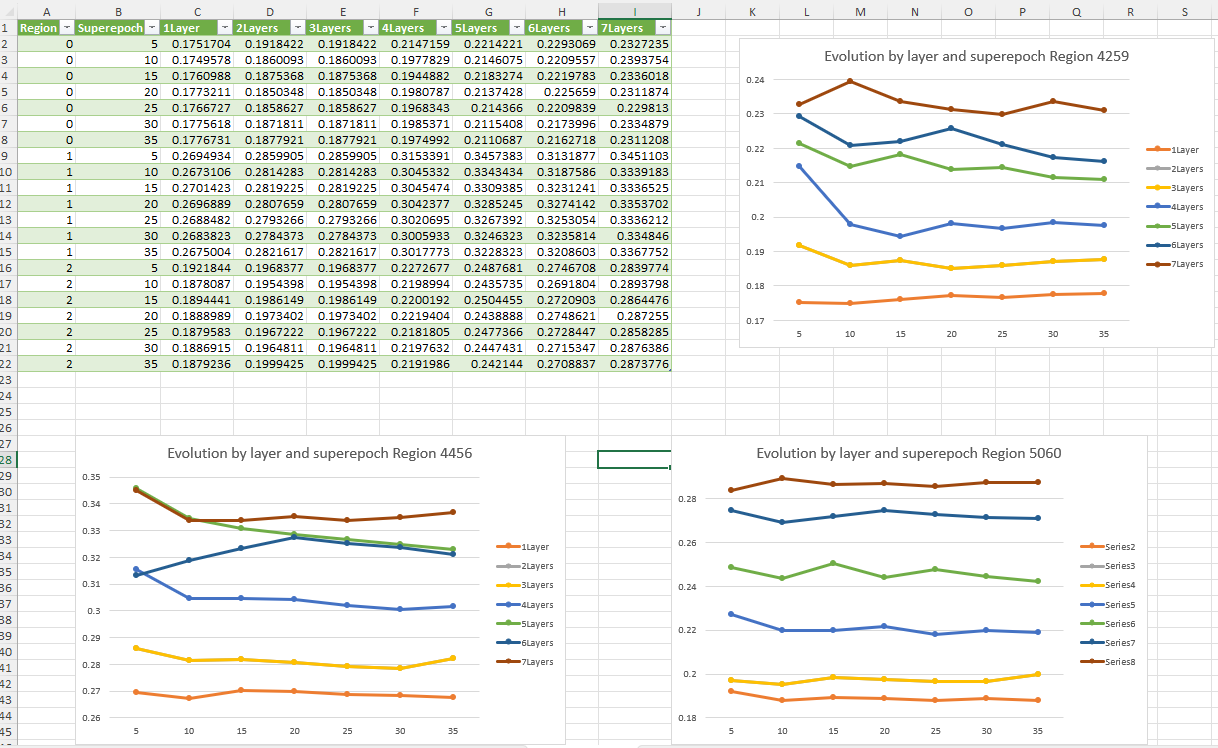
\includegraphics[width=\linewidth]{3x1/LayerTest/train_3x1.PNG}
    \caption{RNMSE de entrenamiento 3 celdas}
    \label{fig1:train3x1}
\end{figure}

\begin{figure}[h!]
    \centering
    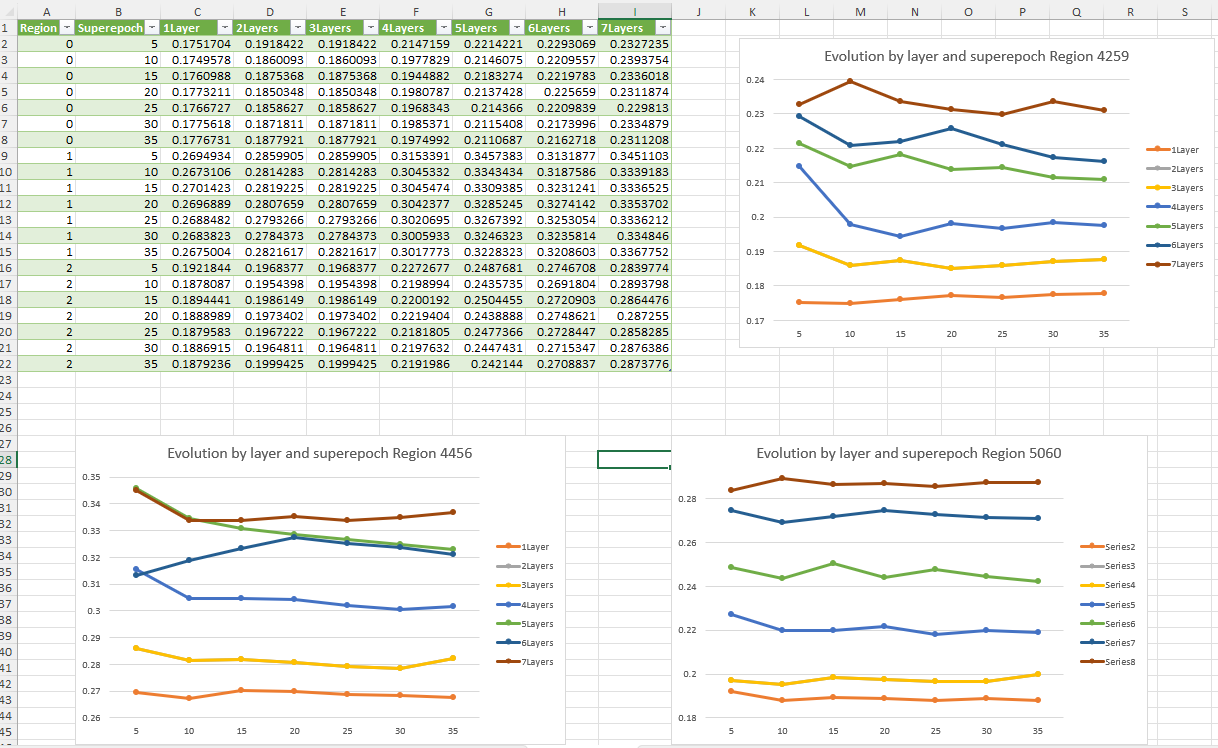
\includegraphics[width=\linewidth]{3x1/LayerTest/train_3x1.PNG}
    \caption{RNMSE de test estático 3 celdas}
    \label{fig1:static3x1}
\end{figure}

\begin{figure}[h!]
    \centering
    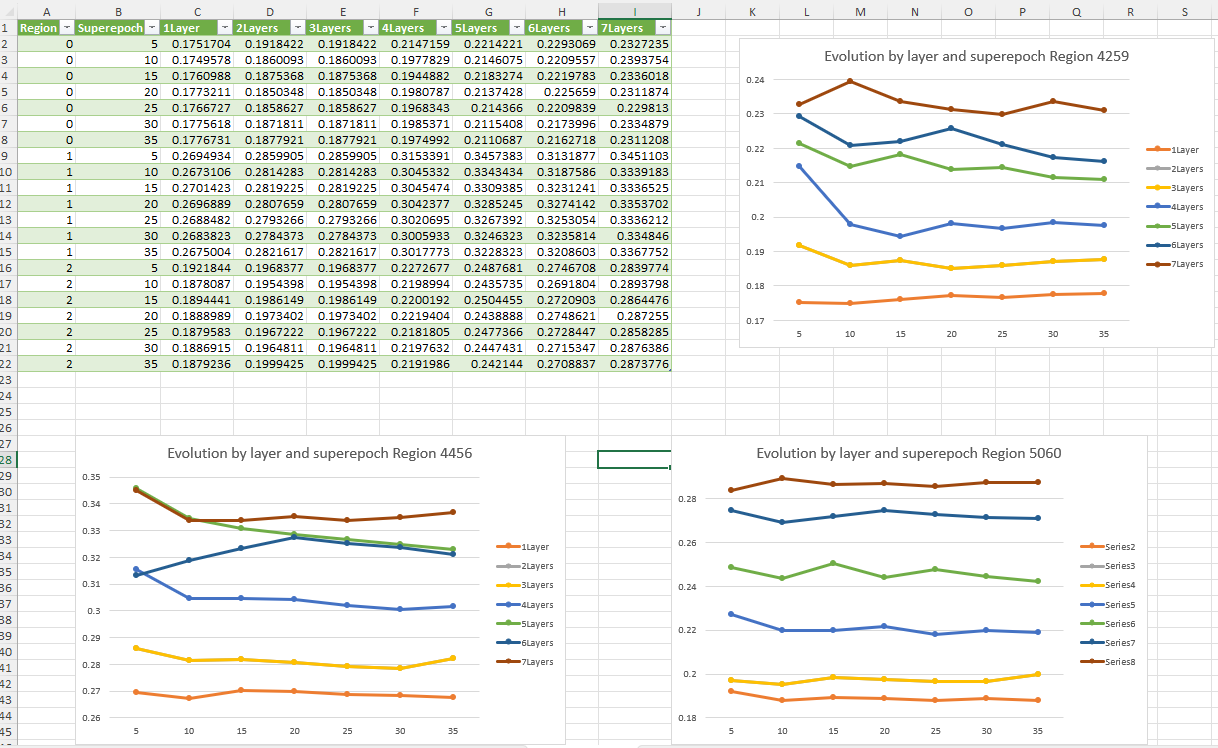
\includegraphics[width=\linewidth]{3x1/LayerTest/train_3x1.PNG}
    \caption{RNMSE de entrenamiento incremental 3 celdas}
    \label{fig1:incremental3x1}
\end{figure}






\FloatBarrier
\subsection{7x7 LSTM}
El TFG está basado en el uso de una red convolucional (CNN) en una zona de 49 celdas de tráfico dispuestas en un cuadrado de 7x7 celdas contiguas. Por ello he decidido no pasar mucho tiempo entrenando una red neuronal de 3 celdas separadas entre sí.

Primeramente he entrenado una red neuronal compuesta sólamente por una capa de LSTM, inluyendo claramente una capa de entrada (\texttt{Input}) y una de salida (\texttt{Dense}).

\begin{lstlisting}[style=pythonstyle, caption={Capas de la red 7x7LSTM}]
    myLSTM = Sequential()
    myLSTM.add(Input(batch_shape=(batch_size, trainX.shape[1], trainX.shape[2])))
    myLSTM.add(LSTM(look_back, stateful=True))
    myLSTM.add(Dense(trainX.shape[2]))
    myLSTM.compile(loss='mean_squared_error', optimizer='adam')
    myLSTM.summary()
\end{lstlisting}


\subsubsection{Resultados}
Por ahora, sin haber conseguido reproducibilidad, he ejecutado el Grid Search 3 veces. Cuando los ejecuté pensé que sería reproducible, por lo que en la segunda y tercera ejecución usé los hiperparámetros que mejor lo hicieron en las anteriores ejecuciones. Para evaluarlas, calculé la media del RNMSE de cada celda en cada combinación de hiperparámetros y comparé el error en el entrenamiento incremental, que es el que interesa para el TFG.

La primera ejecución busqué afinar el tamaño de la ventana \texttt{lookback} y el tamaño del \textit{batch}, siendo los mejores valores \texttt{lookback}=12 y 24 horas y \texttt{batchsize}=25. También descarté actualizar los pesos sólo 3 veces con cada nuevo dato (\texttt{n\_epoch\_updates}) y usar un \texttt{threshold} mayor al 20\%.

En la segunda ví que la ventana \texttt{lookback} se podía reducir a 16 y 20 horas, actualizar los pesos entre 6 y 7 veces con cada nuevo dato y usar un \texttt{threshold} entre 12 y 14\%.

En la tercera probé a afinar el tamaño del \textit{batch}, consiguiendo el óptimo entre 22 y 23 ventanas.

Con dichos resultados, como varias combinaciones de parámetros estaban repetidas entre una y otra ejecución, pude comprobar que no eran resultados reproducibles. La diferencia de resultados era de incluso el 10\% de RNMSE, lo que es absolutamente inaceptable.

\subsection{7x7 CNN-LSTM}
Después he añadido una capa de CNN para extraer la correlación espacial entre las celdas y así la capa LSTM tenga más información para realizar sus predicciones.

Para conectar la red CNN con la red LSTM he introducido una capa de tipo \texttt{Flatten}, que cambia el formato de la salida de la CNN para adaptarlo a la entrada de la LSTM. La CNN produce una salida del tipo (\textit{width, height, filters}) pero la LSTM requiere un vector de entrada en una dimensión. La capa \texttt{Flatten} no aprende nada ni ajusta pesos, sólo cambia la forma de los vectores.

\begin{lstlisting}[style=pythonstyle, caption={Añadido enable\_op\_determinism()}]


    # CNN-LSTM MODEL (Keras 3 Compliant)
    myCNNLSTM = Sequential()
    myCNNLSTM.add(Input(batch_shape=(batch_size, look_back, 7, 7, 1)))
    myCNNLSTM.add(TimeDistributed(Conv2D(filters=current_filters, kernel_size=(3,3), padding='same', activation='relu')))
    myCNNLSTM.add(TimeDistributed(Flatten())) # Flatten to connect CNN to LSTM
    myCNNLSTM.add(LSTM(look_back, stateful=True))
    myCNNLSTM.add(Dense(num_features))
    myCNNLSTM.compile(loss='mean_squared_error', optimizer='adam')

\end{lstlisting}

He descartado con unas simulaciones iniciales y con un poco de lógica aumentar el número de capas. La red es perfectamente capaz de seguir los patrones con una sola capa LSTM.

\subsubsection{Resultados}
Tras ejecutar varias veces el script de Grid Search no parece que haya una mejoría notable en los resultados de la red neuronal CNNLSTM frente a sólo LSTM. Además, el tiempo de procesado aumenta bastante y por si no fuera poco, los resultados no son reproducibles.

Como en la red 7x7LSTM, he intentado ir afinando los hiperparámetros: una ventana de 24 horas, \textit{batches} de 25 ventanas, \texttt{threshold} del 5\%, \texttt{n\_epoch\_updates} entre 5 y 7 y entre 16 y 20 filtros para la capa convolucional.




\section{Simulaciones con reproducibilidad}

\subsection{Resultados 7x7 LSTM}
He utilizado un Grid Search con pocos valores puesto que era una prueba de reproducibilidad y suponía que la velocidad de procesamiento se vería afectada (alrededor de 8 horas de procesado).

He probado los siguientes valores:
\begin{lstlisting}[style=pythonstyle, caption={Grid Search LSTM reproducible}]
#Parameter tweak
hyperparameters = {
    'look_back': [16, 18],
    'batch_size': [22, 23, 24],
    'n_epochs_update': [6, 7],
    'threshold': [0.13, 0.15],
}
\end{lstlisting}

Dichos valores están sacados de las pruebas que realicé cuando el código no era reproducible. Los resultados se encuentran en las Tablas \ref{tab:LSTMrepro1} y \ref{tab:LSTMrepro2}. Como se puede observar, lo único que varía es el tiempo medio que tarda la red en procesar un \textit{batch} en el entrenamiento incremental.

Ahora que sé que es reproducible, volveré a probar otros valores para tener las medidas correctas.

\begin{longtable}[h!]{cccccccc}
	\caption{Resultados de la simulación nº1 7x7 LSTM (LB=\textit{lookback} BS=\textit{batchsize} NEU=\textit{n\_epoch\_updates} TH=\textit{threshold})}\\
	\label{tab:LSTMrepro1}\\


	\toprule
	\textbf{LB} & \textbf{BS} & \textbf{NEU} & \textbf{TH} & \textbf{Train} & \textbf{Static} & \textbf{Online} & \textbf{Time}\\
	\midrule
	\endfirsthead

	\toprule
	\textbf{LB} & \textbf{BS} & \textbf{NEU} & \textbf{TH} & \textbf{Train} & \textbf{Static} & \textbf{Online} &\textbf{Time}\\
	\midrule
	\endhead

	\bottomrule
	\endfoot

	% Data block
	\csvreader[head to column names]{7x7/ReproTest/GridSearch_LSTM_fast_r_v1.csv}{}{
		\lookback & \batchsize & \updates & \threshold & \AvgTrainRNMSE & \AvgTestRNMSE & \AvgTestIncRNMSE & \AvgTestIncTime \\
	}
\end{longtable}

\begin{longtable}[h!]{cccccccc}
	\caption{Resultados de la simulación nº2 7x7 LSTM (LB=\textit{lookback} BS=\textit{batchsize} NEU=\textit{n\_epoch\_updates} TH=\textit{threshold})}\\
	\label{tab:LSTMrepro2}\\


	\toprule
	\textbf{LB} & \textbf{BS} & \textbf{NEU} & \textbf{TH} & \textbf{Train} & \textbf{Static} & \textbf{Online} & \textbf{Time}\\
	\midrule
	\endfirsthead

	\toprule
	\textbf{LB} & \textbf{BS} & \textbf{NEU} & \textbf{TH} & \textbf{Train} & \textbf{Static} & \textbf{Online} & \textbf{Time}\\
	\midrule
	\endhead

	\bottomrule
	\endfoot

	% Data block
	\csvreader[head to column names]{7x7/ReproTest/GridSearch_LSTM_fast_r_v1_2.csv}{}{
		\lookback & \batchsize & \updates & \threshold & \AvgTrainRNMSE & \AvgTestRNMSE & \AvgTestIncRNMSE & \AvgTestIncTime \\
	}
\end{longtable}
\FloatBarrier

Los 3 mejores resultados han sido con \texttt{lookback}=18h, \texttt{batch\_size}=[23,24], \texttt{n\_epoch\_updates}=[6,7] y \texttt{threshold}=0.13.

En las combinaciones ganadoras el test estático ha tenido un 10\% más de RNMSE que el entrenamiento incremental, estando el test estático alrededor de 0.31 y el entrenamiento incremental alrededor de 0.23. Sin embargo, el entrenamiento incremental tiene una varianza mayor a lo largo de las diferentes combinaciones, variando entre 0.21 y 0.518, mientras el test estático se mantiene prácticamente constante independientemente de los hiperparámetros.


\FloatBarrier

\subsection{Resultados CNN+LSTM}
También he utilizado un Grid Search con pocos valores sacados de las simulaciones no reproducibles puesto que era una prueba de reproducibilidad y suponía que la velocidad de procesamiento se vería afectada (alrededor de 17 horas de procesado).

He probado los siguientes valores:
\begin{lstlisting}[style=pythonstyle, caption={Grid Search CNN+LSTM reproducible}]
#Parameter tweak
hyperparameters = {
    'look_back': [12, 24],
    'batch_size': [20, 25],
    'n_epochs_update': [6, 7],
    'threshold': [0, 0.1],
    'num_filters': [16, 20]
}
\end{lstlisting}

Los resultados son reproducibles pero no muy esperanzadores, mostrados en las Tablas \ref{tab:CNNLSTMrepro1} y \ref{tab:CNNLSTMrepro2}. He conseguido la reproducibilidad ya que lo único que varía es el tiempo de procesado medio de un \textit{batch} en el entrenamiento incremental.

\begin{longtable}[h!]{ccccccccc}
	\caption{Resultados de la simulación nº1 7x7 CNN+LSTM (LB=\textit{lookback} BS=\textit{batchsize} NEU=\textit{n\_epoch\_updates} TH=\textit{threshold} NF=\textit{número filtros})}\\
	\label{tab:CNNLSTMrepro1}\\


	\toprule
	\textbf{LB} & \textbf{BS} & \textbf{NEU} & \textbf{TH} & \textbf{NF} & \textbf{Train} & \textbf{Static} & \textbf{Online} & \textbf{Time} \\
	\midrule
	\endfirsthead

	\toprule
	\textbf{LB} & \textbf{BS} & \textbf{NEU} & \textbf{TH} & \textbf{NF} & \textbf{Train} & \textbf{Static} & \textbf{Online} & \textbf{Time} \\
	\midrule
	\endhead

	\bottomrule
	\endfoot

	% Data block
	\csvreader[head to column names]{CNNLSTM/ReproTest/GridSearch_CNNLSTM_repro1.csv}{}{%
		\lookback & \batchsize & \updates & \threshold & \numfilters & \AvgTrainRNMSE & \AvgTestRNMSE & \AvgTestIncRNMSE & \AvgTestIncTime \\
	}

\end{longtable}
\FloatBarrier

\begin{longtable}[h!]{ccccccccc}
	\caption{Resultados de la simulación nº2 7x7 CNN+LSTM (LB=\textit{lookback} BS=\textit{batchsize} NEU=\textit{n\_epoch\_updates} TH=\textit{threshold} NF=\textit{número filtros})}\\
	\label{tab:CNNLSTMrepro2}\\


	\toprule
	\textbf{LB} & \textbf{BS} & \textbf{NEU} & \textbf{TH} & \textbf{NF} & \textbf{Train} & \textbf{Static} & \textbf{Online} & \textbf{Time} \\
	\midrule
	\endfirsthead

	\toprule
	\textbf{LB} & \textbf{BS} & \textbf{NEU} & \textbf{TH} & \textbf{NF} & \textbf{Train} & \textbf{Static} & \textbf{Online} & \textbf{Time} \\
	\midrule
	\endhead

	\bottomrule
	\endfoot

	% Data block
	\csvreader[head to column names]{CNNLSTM/ReproTest/GridSearch_CNNLSTM_repro2.csv}{}{%
		\lookback & \batchsize & \updates & \threshold & \numfilters & \AvgTrainRNMSE & \AvgTestRNMSE & \AvgTestIncRNMSE & \AvgTestIncTime \\
	}

\end{longtable}
\FloatBarrier

 Los 3 mejores resultados fueron con \texttt{lookback}=24h, batch\_size=25, n\_epochs\_update=[6,7], \texttt{threshold} =[0,0.1] y entre 16 y 20 filtros. Los resultados no han supuesto una mejora respecto a la red neuronal LSTM. El valor del RNMSE de CNN+LSTM en cuanto a entrenamiento incremental es muy parecido sin llegar a superar el de LSTM.

Cabe destacar que con la red CNN el RNMSE del entrenamiento incremental es más estable entre combinaciones de hiperparámetros que con sólo la red LSTM.


\section{Grid Search extendido con aumento de velocidad}
He realizado un Grid Search más exhaustivo, detallado en la Tabla \ref{tab:CNNLSTMextended}. Como la reproducibilidad ya está implementada, este Grid Search no contiene las combinaciones de las Tablas \ref{tab:CNNLSTMrepro1} y \ref{tab:CNNLSTMrepro2}.

Los mejores resultados han sido: \textit{lookback}=24, aunque \textit{lookback}=18 parece ser mejor que \textit{lookback}=12; \textit{batchsize}=23, \textit{n\_epoch\_updates}=6, \textit{threshold}=10\%, destacando que la ausencia de \textit{threshold} también da muy buenos resultados independientemente del resto de hiperparámetros y un \textit{threshold} demasiado elevado no es viable; \textit{num\_filters}=16.

\begin{longtable}[h!]{ccccccccc}
	\caption{Resultados de la simulación con Grid Search extendido 7x7 CNN+LSTM y mejoras de velocidad (LB=\textit{lookback} BS=\textit{batchsize} NEU=\textit{n\_epoch\_updates} TH=\textit{threshold} NF=\textit{número filtros})}\\
	\label{tab:CNNLSTMextended}\\


	\toprule
	\textbf{LB} & \textbf{BS} & \textbf{NEU} & \textbf{TH} & \textbf{NF} & \textbf{Train} & \textbf{Static} & \textbf{Online} & \textbf{Time} \\
	\midrule
	\endfirsthead

	\toprule
	\textbf{LB} & \textbf{BS} & \textbf{NEU} & \textbf{TH} & \textbf{NF} & \textbf{Train} & \textbf{Static} & \textbf{Online} & \textbf{Time} \\
	\midrule
	\endhead

	\bottomrule
	\endfoot

	% Data block
	\csvreader[head to column names]{CNNLSTM/GridSearch_CNNLSTM_extended.csv}{}{%
		\lookback & \batchsize & \updates & \threshold & \numfilters & \AvgTrainRNMSE & \AvgTestRNMSE & \AvgTestIncRNMSE & \AvgTestIncTime \\
	}

\end{longtable}
\FloatBarrier

\subsection{Mejoras de velocidad}
Los resultados de la Tabla \ref{tab:CNNLSTMextended} fueron obtenidos tras modificar el código de la red CNN+LSTM para aumentar la velocidad de procesamiento. La primera mejora pasa por evitar que Keras tenga que reorganizar la memoria de la GPU cada vez que se llama a la función \texttt{.fit()}. Esto se evita utilizando un \texttt{Callback} en la llamada a la función \texttt{.fit()}, forzando a Keras a organizar la memoria de la GPU una sola vez, mandando a la GPU la orden de realizar todas las iteraciones del bucle en una sola llamada. Así, el bucle que llama a la función \texttt{.fit()} un total de \texttt{n\_epochs} veces queda de la forma:

\begin{lstlisting}[style=pythonstyle, caption={\texttt{Callback} para la función \texttt{.fit()}}]
#Callback para la funcion .fit()
class ResetStatesCallback(tf.keras.callbacks.Callback):
	def on_epoch_end(self, epoch, logs=None):
		for layer in self.model.layers:
			if hasattr(layer, 'reset_states'):
				layer.reset_states()


#El bucle se transforma en una unica llamada a la funcion .fit()
myCNNLSTM.fit(
	trainX, trainY,
	epochs=n_epochs,
	batch_size=batch_size,
	verbose=0,
	shuffle=True,
	callbacks=[ResetStatesCallback()] # Callback para .fit()
)
\end{lstlisting}

La segunda mejora se encuentra en la parte de entrenamiento incremental. También está basada en evitar que el intérprete de Python tenga que hacer demasiadas llamadas a la GPU. En este caso he invocado al compilador \texttt{AutoGraph} mediante \texttt{@tf.function}, que transforma el código de Python en operaciones matemáticas optimizadas de \texttt{Tensorflow}. Además, utiliza \texttt{Accelerated Linear Algebra (XLA)} y \texttt{Kernel Fusion} para simplificar las operaciones matemáticas en un único comando para la GPU.


\begin{lstlisting}[style=pythonstyle, caption={Uso de \texttt{AutoGraph}, \texttt{XLA} y \texttt{Kernel Fusion} mediante \texttt{@tf.function}}]
@tf.function	#Invocar AutoGraph, XLA y Kernel Fusion
def skima_train_step(model, optimizer, x, y, norm_sq):
	with tf.GradientTape() as tape:
		predictions = model(x, training=True)
		loss = rmse_loss(y, predictions)

	gradients = tape.gradient(loss, model.trainable_variables)
	adjuted_gradients = [g * norm_sq for g in gradients]
	optimizer.apply_gradients(zip(adjusted_gradients, model.trainable_variables))


# Uso de la funcion skima_train_step()
if rmse_norm > error_threshold:
	st = tt.time()

	#RMSE_NORM como tensor para AutoGraph
	norm_sq_tensor = tf.cast(rmse_norm**2, tf.float32)

	for j in range(n_epochs_update):
		# Uso de XLA y Kernel Fusion
		skima_train_step(myCNNLSTM, optimizer, online_X, online_Y, norm_sq_tensor)

	# Resetear los estados
	for layer in myCNNLSTM.layers:
		if hasattr(layer, 'reset_states'):
			layer.reset_states()

	et = tt.time()
	.
	.
	.
\end{lstlisting}
\FloatBarrier

El último Grid Search, descrito en la Tabla \ref{tab:CNNLSTMextended}, se realizó con las mejoras de velocidad aquí descritas. Tardó 43200.4 segundos en procesar todas sus combinaciones. Por su parte, el Grid Search anterior, descrito en la Tabla \ref{tab:CNNLSTMrepro2}, tardó 34459.3 segundos. Las mejoras introducidas merecen mucho la pena, como se puede observar en la columna \textbf{Time} de la Tabla \ref{tab:CNNLSTMextended}.

\begin{align*}
	43200.4/(3*3*3*3*3-2*2*2*2*2)&=204.74 \; segundos/combinacion \; con \; mejora\\
	34459.3/(1*3*3*3*3)&=1076.85 \: segundos/combinacion \; sin \; mejora
\end{align*}

Para comprobar que estas mejoras de velocidad no hubiesen comprometido la reproducibilidad, he realizado de nuevo una parte del último Grid Search, detallado en la Tabla\ref{tab:CNNLSTMextendedrepro} y he comprobado que la reproducibilidad se ha visto afectada en lo más mínimo.

\begin{longtable}[h!]{ccccccccc}
	\caption{Resultados de la prueba de reproducibilidad con Grid Search extendido 7x7 CNN+LSTM con mejoras de velocidad (LB=\textit{lookback} BS=\textit{batchsize} NEU=\textit{n\_epoch\_updates} TH=\textit{threshold} NF=\textit{número filtros})}\\
	\label{tab:CNNLSTMextendedrepro}\\


	\toprule
	\textbf{LB} & \textbf{BS} & \textbf{NEU} & \textbf{TH} & \textbf{NF} & \textbf{Train} & \textbf{Static} & \textbf{Online} & \textbf{Time} \\
	\midrule
	\endfirsthead

	\toprule
	\textbf{LB} & \textbf{BS} & \textbf{NEU} & \textbf{TH} & \textbf{NF} & \textbf{Train} & \textbf{Static} & \textbf{Online} & \textbf{Time} \\
	\midrule
	\endhead

	\bottomrule
	\endfoot

	% Data block
	\csvreader[head to column names]{CNNLSTM/GridSearch_CNNLSTM_extendedrepro.csv}{}{%
		\lookback & \batchsize & \updates & \threshold & \numfilters & \AvgTrainRNMSE & \AvgTestRNMSE & \AvgTestIncRNMSE & \AvgTestIncTime \\
	}

\end{longtable}
\FloatBarrier


\section{Resultados CNN+CNN+LSTM}
He aumentado el número de capas de la red neuronal CNN y probado con el siguiente set de 972 combinaciones de hiperparámetros:

\begin{lstlisting}[style=pythonstyle, caption={Grid Search CNN+CNN+LSTM reproducible}]
	#Parameter tweak
	hyperparameters = {
		'look_back': [18, 20, 24],
		'batch_size': [23, 25, 27],
		'n_epochs_update': [5, 6, 7],
		'threshold': [0, 0.1, 0.15, 0.2],
		'num_filters1': [12, 14, 16],
		'num_filters2': [20, 22, 24]
	}
\end{lstlisting}

Siendo \texttt{num\_filters1} el número de filtros de la primera capa y \texttt{num\_filters2} el número de filtros de la segunda capa. Visto que la primera capa analiza los datos para extraer patrones básicos, he considerado darle menos filtros que a la segunda capa, que debe transformar los patrones básicos en patrones más complejos.


Los mejores resultados en cuanto a \texttt{Avg\_Test\_Inc\_Score} fueron:

\begin{table}[h]
	\centering
	\caption{Mejor combinación para la red CNN+CNN+LSTM}
	\begin{tabular}{cccccccccc}
		\toprule
		\textbf{LB} & \textbf{BS} & \textbf{NEU} & \textbf{TH} & \textbf{NF1} & \textbf{NF2} & \textbf{Train} & \textbf{Static} & \textbf{Online} & \textbf{Time} \\
		\midrule
		18 & 25 & 6 & 0.1 & 14 & 20 & 0.122076 & 0.366933 & 0.211242 & 0.065284\\
		\bottomrule
	\end{tabular}
\end{table}

\subsection{Análisis de resultados}
Al tener tantos resultados, no es posible analizarlos a mano. Por ello, para poder identificar las tendencias presentes en los datos, he utilizado el coeficiente de Spearman.

Este coeficiente permite encontrar tendencias en los datos sin necesidad de que estas tendencias sean estrictamente lineales como ocurre con el coeficiente de Pearson. Además, hay suficientes datos como para que se desvanezcan las ventajas del coeficiente de Kendall. Además, el coeficiente de Spearman puede indicar correlaciones proporcionales (signo positivo) o inversamente proporcionales (signo negativo).

En este caso, un signo negativo indica que el error o el tiempo de procesado disminuye cuando el hiperparámetro en cuestión aumenta y viceversa.

\begin{table}[htpb]
	\centering
	\caption{Coeficientes de Correlación de Spearman para CNN+CNN+LSTM}
	\label{tab:spearman_corr}
	\begin{tabular}{|l|c|c|c|c|}
		\hline
		  & \textbf{AvgTrainRNMSE} & \textbf{AvgTestRNMSE} & \textbf{AvgTestIncRNMSE} & \textbf{AvgTestIncTime} \\ \hline
		\textbf{lookback}       & $-0.121340$            & $0.148394$            & $-0.037053$              & $-0.010026$             \\ \hline
		\textbf{batchsize}      & $0.266828$             & $-0.047088$           & $0.018862$               & $-0.275763$             \\ \hline
		\textbf{updates}        & $-0.020447$            & $0.007675$            & $-0.150139$              & $0.828263$              \\ \hline
		\textbf{threshold}      & $0.022866$             & $0.007318$            & $-0.003070$              & $-0.030932$             \\ \hline
		\textbf{numfilters1}    & $-0.077155$            & $0.028489$            & $-0.093504$              & $0.046299$              \\ \hline
		\textbf{numfilters2}    & $-0.345310$            & $-0.156740$           & $-0.046374$              & $0.032351$              \\ \hline
	\end{tabular}
\end{table}

Un coeficiente de Spearman menor a 0.05 es considerado como una ausencia de correlación. Así, los hiperparámetros que influyen en el rendimiento del entrenamiento incremental son \texttt{n\_epoch\_updates} y \texttt{num\_filters1}. Tiene sentido cuantas más veces se reentrene la red neuronal con el nuevo dato obtenido (\texttt{n\_epoch\_updates}), menor sea el error puesto que la red neuronal tiene más posibilidades de adaptarse al nuevo dato. También, al añadir más filtros en la primera capa CNN, la red puede extraer más patrones y usarlos para las predicciones. Es interesante ver que el número de filtros de la segunda capa no tiene un impacto predecible en el entrenamiento incremental.

Para el test convencional, los hiperparámetros con una tendencia visible son el número de muestras que la red procesa al mismo tiempo y el número de filtros de la segunda capa CNN. No encuentro mucha justificación a esto. Porbablemente al subir el número de muestras (ventana) que la red procesa a un mismo tiempo haga que la red no extraiga bien el patrón de dicha ventana pero no es una explicación plausible con la correlación inversa que tiene \texttt{look\_back} con el error de entrenamiento. Otra explicación probable es que aumentar el tamaño de la ventana provoque un pequeño efecto de \textit{overfitting}, lo que explicaría la relación inversa con el error de entrenamiento y la relación directa con el error de test. Respecto a los filtros de la segunda capa tampoco tengo una expliación coherente. ¿Por qué los filtros de la segunda sí y los de la primera no? ¿Por qué en el entrenamiento incremental es al revés? Sinceramente no tengo respuesta todavía. De todas formas, tienen coeficientes de Spearman relativamente bajos.

%% SPEARMAN NF1 AVGTESTINCRNMSE ES DESPRECIABLE


Respecto al entrenamiento, un aumento del tamaño de los \textit{batches} produce una caída del rendimiento, seguramente porque al aumentar el tamaño de los batches hay menos batches en el dataset y el entrenamiento es menos intensivo. Con el número de filtros de las capas CNN pasa lo mismo que con el rendimiento en test aunque esta vez un coeficiente de Spearman de -0.345 no es despreciable.

Respecto al tiempo de procesado del entrenamiento incremental tiene unos coeficientes de Spearman previsibles. Al aumentar el número de veces que se reentrena la red con un mismo dato (\texttt{n\_epoch\_update}) aumenta el tiempo que tarda. Cando aumenta el tamaño del \textit{batch}, las GPU pueden procesar más datos en paralelo. En cuanto al hiperparámetro \texttt{threshold}, hay que tener en cuenta que sólo se computan y se tienen en cuenta los tiempos en los cuales el error de la red es mayor al threshold y se ejecuta el entrenamiento incremental. Cuando el \texttt{threshold} no permite que se realice el entrenamiento incremental el tiempo de ejecución \texttt{TestIncTime} es 0 pero no se tiene en cuenta para el \texttt{AvgTestIncTime} puesto que daría resultados muy cercanos a cero y se perdería la información de el tiempo que realmente tarda el entrenamiento incremental en asumir un dato nuevo.



\section{Resultados CNN+CNN+CNN+LSTM}
También he realizado pruebas con 3 capas de CNN. He probado con el siguiente set de combinaciones de hiperparámetros:

\begin{lstlisting}[style=pythonstyle, caption={Grid Search CNN+CNN+CNN+LSTM}]
	#Parameter tweak
	hyperparameters = {
		'look_back': [18, 24],
		'batch_size': [23, 25],
		'n_epochs_update': [5, 6, 7],
		'threshold': [0, 0.1],
		'num_filters1': [12, 14, 16],
		'num_filters2': [20, 22, 24],
		'num_filters3': [26, 28, 30]
	}
\end{lstlisting}

Todavía no he completado el \textit{Grid search} puesto que tarda mucho en procesar pero por ahora el ganador es:

\begin{table}[h]
	\centering
	\caption{Mejor combinación para la red CNN+CNN+LSTM}
	\begin{tabular}{ccccccccccc}
		\toprule
		\textbf{LB} & \textbf{BS} & \textbf{NEU} & \textbf{TH} & \textbf{NF1} & \textbf{NF2} & \textbf{NF3} & \textbf{Train} & \textbf{Static} & \textbf{Online} & \textbf{Time} \\
		\midrule
		18 & 25 & 6 & 0 & 12 & 24 & 28 & 0.11261 & 0.32942 & 0.213898 & 0.073121\\
		\bottomrule
	\end{tabular}
\end{table}

Aunque hay una capa más de CNN, los resultados no han sido mejores que con sólo 2 capas aunque están cerca. Además de ser una red más compleja y costosa de entrenar.

No creo que añadir una cuarta capa sea beneficioso para un \textit{grid} de 7x7.  Con un \textit{kernel} de 3x3, la cuarta capa sólo necesitaría una celda para recoger información de todas las 49 celdas al mismo tiempo.

Tampoco creo que añadir capas de \textit{pooling} sea algo beneficioso. Después de todo, un \textit{grid} de 7x7 es relativamente pequeño y una capa de \textit{pooling} puede dejar a la red neuronal sin datos. Además, añadir capas de CNN tiene la intención de proporcionar a la red datos acerca de las relaciones espaciales entre las celdas. Si añado una capa de \textit{pooling} estoy destruyendo esa información.


\section{Acciones futuras}
Terminar el \textit{Grid Search} de 3CNN + LSTM. Además, realizar el análisis de Spearman.

Realizar una pequeña prueba añadiendo una \textit{pooling layer} en la red 2CNN+LSTM.

Empezar a redactar la memoria del TFG.

\end{document}


